Eine große Herausforderung bei der Modellierung des Softwareentwicklungsprozesses war eine genaue Momentaufnahme eines kontinierlichen arbeitenden Prozesses. 

\begin{figure}[p]
    \centering
    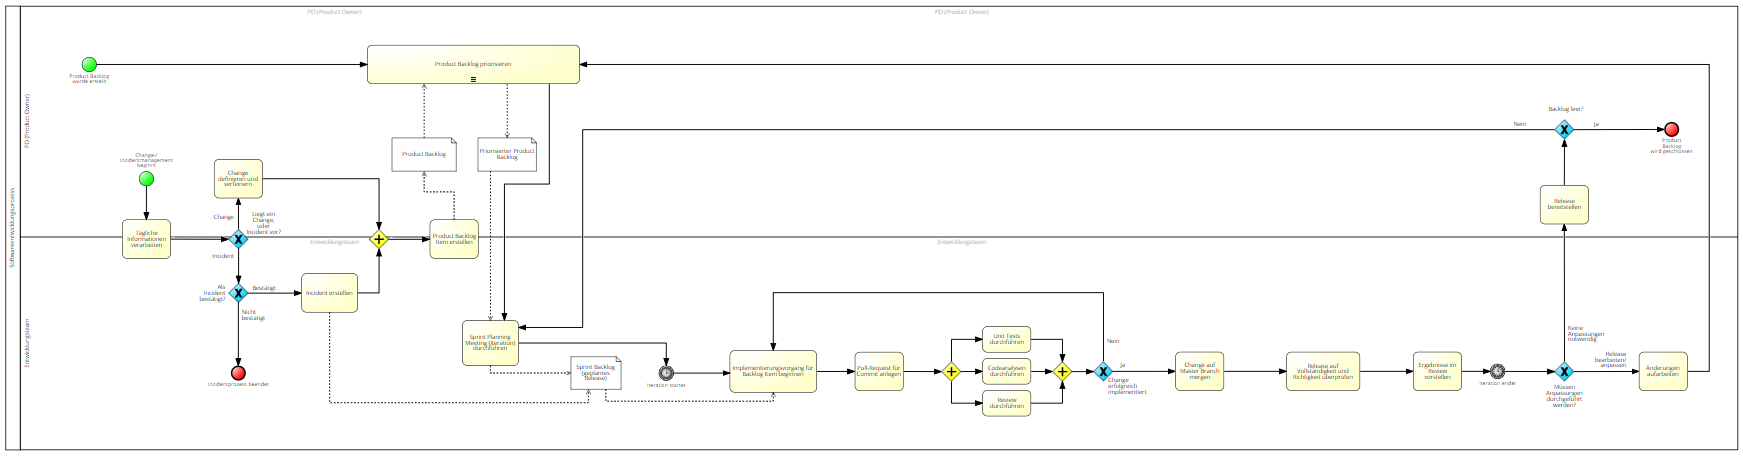
\includegraphics[angle=90, scale=0.6]{Bilder/IST-Prozess_neu.png}
    \caption{Softwareentwicklungsprozess im IST-Zustand basierend auf dem internen msg-Projekt}
\end{figure}

Im Rahmen dieser Arbeit bildet die Grundlage des vorgestellten Prozesses, der Softwareentwicklungsprozess basierend auf dem internen Projekt innerhalb der msg systems ag, ab.

Dieser Prozess beschreibt die Vorgehensweise und die darauf aufbauenden Aufgaben, die im Laufe der Entwicklung zu erbringen sind und an dem konkreten Projekt festgelegt wurden.

Da das entsprechende Team mit agilen Methoden wie Scrum und Kanban und mittels DevOps-Methoden arbeitet, erwies sich die Modellierung des IST-Prozesses basierend auf einem Sprint am geeignesten. 

Da die Rollen von DevOps, sowohl den Tätigkeitsbereich als auch den entsprechenden Personenrahmen abbilden, werden die Aufgaben innerhalb DevOps als eine zusammenhängende und eigenständige Rolle behandelt und trägt daher den Namen 'Entwicklungsteam'.

Somit entsprechen innerhalb dieses konkreten Projektes Dev und Ops, Entwicklern und nehmen infolgedessen beide Tätigkeitsbereiche, also die Entwicklung als auch die Verwaltung, gemeinsam wahr.

Ferner fungiert der Product Owner, als die nächste Rolle, als die Schnittstelle zwischen verschiedenen Stakeholdern oder Kunden und dem Entwicklungsteam. 

Er vertritt demnach die Interessen des Kunden in den Entwicklungsprozess, ohne aktiv in die Softwareentwicklung einzugreifen.

Ferner erstellt der Product Owner den Product Backlog und legt die Reihenfolge der Items, die bearbeitet werden müssen, fest. 

Zum besseren Verständnis wurde der Gesamtprozess in drei Teile (Abbildung 10 - 12) unterteilt und diese einzeln erläutert.\\

\begin{figure}[h]
    \centering
    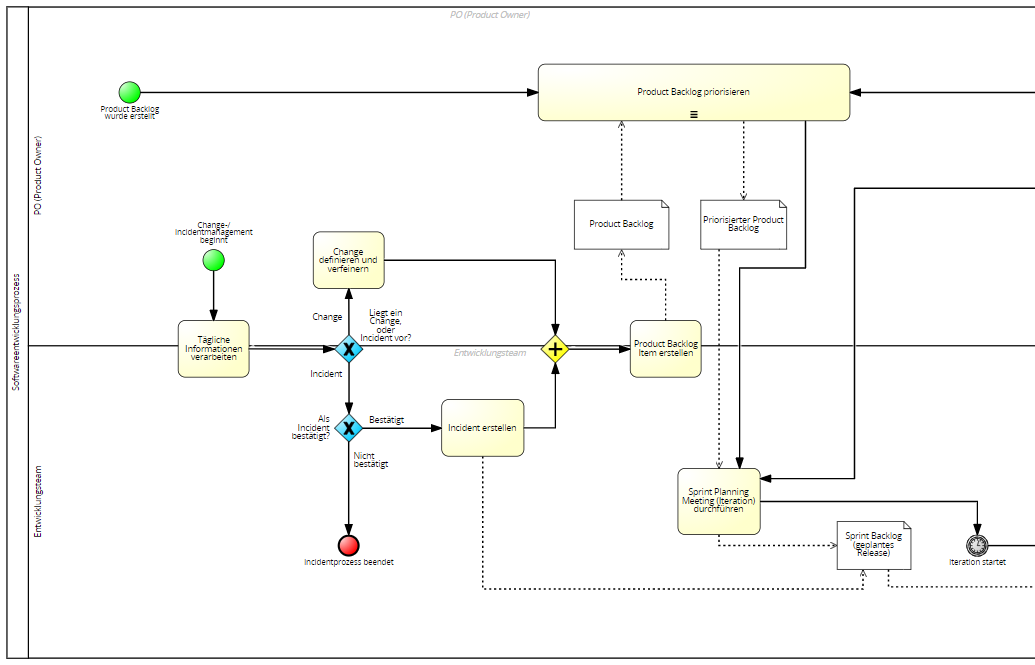
\includegraphics[scale=0.5]{Bilder/IST-Prozess_first Part.png}
    \caption{Erster Teil des Softwareentwicklungsprozess im IST-Zustand basierend auf dem internen msg-Projekt}
\end{figure}

Der erste Startpunkt des Prozesses stellt die Erstellung des Product Backlogs durch den Product Owner dar, welches durchgängig priorisiert und innerhalb der Abbildung 10 dargestellt wird. 

Die Priorisierung findet sequentiell statt, da mehrere Entwicklungen und Änderungen eines Items des Product Backlogs parallel und gleichzeitig und nicht als eine Aufgabenschleife stattfinden. 

Das Ergebnis ist das priorisierte Product Backlog, welches eine Liste der Anforderungen für alle Produktänderungen darstellt, die anhand einer Schätzung in eine abzuarbeitende Reihenfolge gebracht werden. 

Ist die Priorisierung erfolgt, startet die Iteration mit dem Sprint Planning Meeting. 

Hierbei wird abhängig von den verfügbaren Kapazitäten und den Ergebnissen des letzten Sprints entschieden, welche User Stories zuerst bearbeitet werden. 

Sowohl die erstellten Incidents, die als sehr dringend gelten und sofort beseitigt werden müssen, als auch die ausgewählten User Stories des Product Backlogs bilden den Sprint Backlog, welcher somit die geplanten Umsetzungen an Entwicklungen innerhalb des Releases darstellt.

Parallel hierzu beginnt der Change-/Incidentprozess, bei dem zunächst die täglichen Informationen verarbeitet werden. 

Diese Unterprozesse sind essentiell für den Gesamtprozess, da die entsprechenden Ergebnisse aller Unterprozesse zu einer möglichen Codeänderung und infolgedessen zu einer Verwendung von OSS führen können. 

Die Auswirkungen erstrecken sich daher auf den Product Backlog aus, indem festgelegt wird, welche geplanten oder ungeplanten Änderungen zu den bestehenden Anfoderungen am Produkt entwickelt werden müssen und bestimmen daher einen wesentlichen Teil des Inhalts des Product Backlogs.  

Wesentlicher Unterschied beider Prozesse ist, dass der Change eine geplante Veränderung voraussetzt, während der Incident eine ungeplante Entwicklung beansprucht.  

Der Changeprozess bescheibt den Prozess für eine Änderung, die sich auf eine geplante Modifikation der Definition eines bestehenden oder neuen Produkts bezieht und für die das DevOps-Teams verantwortlich ist. 

Der Prozess umfasst die Erfassung jedes Requests, die Dokumentation, Genehmigung und Kontrolle und stellt sicher, dass Change Requests definiert, geplant, effizient, wirtschaftlich und mit vertretbarem Risiko abgewickelt werden. 

Ein Ziel des Change Managements ist es, die Nachvollziehbarkeit von Anforderungen und Änderungen zu gewährleisten.

Währenddessen umfasst das Incident Management den gesamten organisatorischen und technischen Prozess für Reaktionen und Maßnahmen auf Störungen des IT-Betriebs.

Das Spektrum möglicher Incidents reicht von Fehlermeldungen durch Anwender bis hin zu automatisierten Alarmen und Warnungen durch das Monitoring.

Das Ziel des Incident Managements ist die Wiederherstellung eines zugesagten Dienstes in einem definierten Prozess und in optimaler Zeit. 

Dies kann auch Umgehungslösungen beinhalten. 

Incident Management deckt keine (neuen) Anforderungen, Wünsche, Anfragen oder ähnliches ab.  

Obwohl der Change- und Incidentprozess vom Product Owner begonnen wird, ist dieser ausschließlich für den Changeprozess verantwortlich. 

Der Incidentprozess wird anhand des täglichen Monitorings vom Entwicklerteam durchgeführt. 

Nach der Verarbeitung der täglichen Informationen, werden die auftretenden Bugs zunächst in Incident und Changeprozesses unterschieden, da beide Prozesse unterschiedlich behandelt werden.

Innerhalb des Changeprozesses werden die Änderungen definiert und verfeinert und die Anforderungen festgelegt, die entwickelt werden müssen. 

Das Ergebnis fließt in den Product Backlog ein, bei dem die Items wiederrum priorisiert werden. 

Sollte der Bug als Incident bestätigt werden, so wird dieser zunächst erstellt. 

Sollte es sich bei dem erstellten Incident um ein schwerwiegendes Problem handeln, der sofort beseitigt werden muss wird dieser zunächst in das Sprint Backlog übertragen.

Dies ist wichtig, da durch dieses Vorgehen Auskunft während des nächsten Sprint darüber gegeben werden kann, wie hoch die Anzahl der Fehlermeldungen oder Störungen aufgrund ausgefallener Systeme ist und demnach eine Anpassung erforderlich macht. 

Sollte ein Problem auftreten, welches eine Codeänderung benötigt aber nicht als dringlich gilt, wird nach der Erstellung des Incidents, dieser als ein Item in der überarbeitete Product Backlog eingetragen. 

Falls die vermeitliche Incident nicht bestätigt wird, wird dieser vermerkt und geschlossen, wodurch der Incidentprozess ab diesem Zeitpunkt als geschlossen gilt. \\ 

\begin{figure}[h]
    \centering
    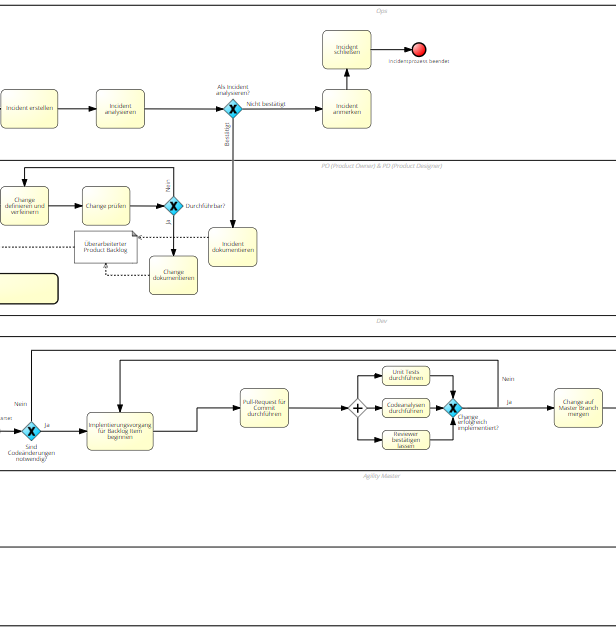
\includegraphics[scale=0.6]{Bilder/IST-Prozess_second Part.png}
    \caption{Zweiter Teil des Softwareentwicklungsprozess im IST-Zustand basierend auf dem internene msg-Projekt}
\end{figure}

Wie in Abbildung 11 zu erkennen ist, startet die Iteration nach dem durchgeführten Sprint Planning Meeting, wodurch der Implmentierungsvorgang für die jeweiligen Sprint Backlog Items beginnen kann. 

In diesem Rahmen sind Codeänderungen notwendig, die sich auf vorhandenen Code oder eine Neuimplementierung beziehen können. 

Je nach Backlog Item entscheidet der Entwickler, welche Maßnahmen durchgeführt werden müssen und dokummentiert etwaige Fehler, die sich während der Entwicklung ergeben können.  

Nachdem der Pull-Request für das Commit durchgeführt wurde, werden mehrere Aufgaben parallel erledigt. 

Dazu gehört die Durchführung der Unit-Test und Codeanalyse und die Bestätigung des Reviewer.

Diese Vorgehensweise ist ebenfalls essentiell für den weiteren Ablauf des Softwareentwicklungsprozesses und beruht auf dem Vier-Augen-Prinzip, um die Qualität und Wartbarkeit sicherzustellen und zu erhöhen.  

Dabei wird ein vorher festgelegter Teil des Quellcodes von Entwicklern, die nicht direkt an der Entwicklung des jeweiligen Codes beteiligt waren, begutachtet und nach Fehlern untersucht. 

Umso später Fehler im Softwareentwicklungsprozesses gefunden werden, desto aufwändiger sind diese zu beheben. 

Darüber hinaus ermöglichen regelmäßige Reviews einen Wissensaustausch, eine Dokumentation über etwaige Schwachstellen und eine kontinierliche Verbesserung der eigenen Kenntnisse, was wiederrum die Kultur von DevOps wiederspiegelt. 

Sollten Fehler gefunden werden oder die Test fehlschlagen, so wird der entsprechende Entwickler informiert. 

Sobald alle Änderungen erfolgreich implementiert worden sind, werden diese auf das Master Branch gemergt. 

\begin{figure}[h]
    \centering
    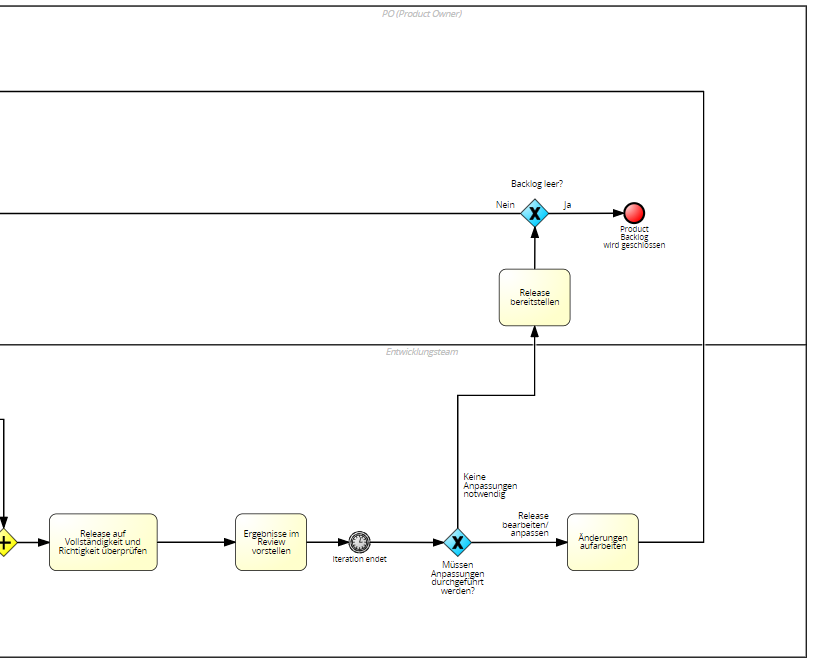
\includegraphics[scale=0.6]{Bilder/IST-Prozess_third Part.png}
    \caption{Dritter Teil des Softwareentwicklungsprozess im IST-Zustand basierend auf dem internen msg-Projekt}
\end{figure}

Nachdem das Mergen erfolgreich durchgeführt wurde, wird das Release auf seine Vollständigkeit und Richtigkeit überprüft und im Review vorgestellt. 

Die Vorstellung erfolgt ebenfalls durch den entsprechenden Entwickler, der die jeweilige Entwicklung den jeweligen Stakeholdern präsentiert. 

Ab diesem Zeitpunkt endet die Iteration. 

Werden weitere Anpassungen benötigt, müssen diese aufgearbeitet werden und fließen in das priorisierte Backlog zurück.

Sind keine Änderungen notwendig, wird das Release bereitgestellt. 

Das Projekt endet sobald das Product Backlog leer ist.

% \paragraph{Agility Master}

% Der Agility Master verantwortet einen effektiven und effizienten Prozess und stellt sicher, dass die Regeln des agil und Lean Management eingehalten werden. 

% Ferner fungiert der Agility Master als ein Moderator für Team-Ereignisse und versucht Probleme und Hindernisse zeitnah zu lösen. 

% Der Agility Master ist mit dem Scrum Master identisch. \dwi{warum führst du dann den namen agility master ein? es hilft dem leser (der nicht aus HAF kommt) nicht, hier einen begriff zu lesen der dann am ende mit einem konzept verglichen wird, das er schon kennt.}

% \paragraph{Dev}

% Diese Rolle entspricht der Rolle des Softwareentwickler oder Development-Teams. 

% Je nach Projektanforderungen kann sich die Rolle des Entwicklers beispielsweise auf das Frontend- oder Backendentwicklung richten.

% \paragraph{Product Owner und Product Designer}
% \dwi{Product Designer ist eine kreation in unserem projekt, und würde in der scrum-welt eher als proxy-po bezeichnet werden. in deinem kontext hilft es aber beides nicht um deine inhalte zu transportieren - nimm nur PO und gut.}

% Zunächst fungiert der Product Owner als die Schnittstelle zwischen verschiedenen Stakeholdern oder Kunden und dem Entwicklungsteam. 

% Er vertritt demnach die Interessen des Kunden in den Entwicklungsprozess, ohne aktiv in die Softwareentwicklung einzugreifen.

% Ferner erstellt der Product Owner den Product Backlog und legt die Reihenfolge der Items, die bearbeitet werden müssen, fest. 

% Wie der Name schon sagt, beschreibt die Rolle des Product Designers die Gestaltung oder den Entwurf des Produkts. 

% Hierzu gehören die Definitionen von UX-Anforderungen und Spezifikationen oder die Schaffung von Schnittstellen, im Hinblick auf die Fuktionalität und das erwartende Verhalten des Produkts. 

% Innerhalb des HAF-Teams überschneiden sich die Rollen des Product Owner und des Product Designers, weshalb diese beiden Positionen in einer Swimlane dargestellt werden.  

% \paragraph{Ops}
% \dwi{du hast jetzt zum einen konkrete rollen die an personen hängen als swimlanes, und dann zwei lanes die an "dev" und "ops" hängen - das sind logische tätigkeitsbereiche. das ist "ungenau". entscheid dich für eine konsistente unterteilung.. und "dev" und "ops" zu trennen ist eigentlich nochmal eine ganz eigene diskussion. vllt kannst die beiden lanes auch zusammenführen unter "developer", sofern du beim rollenbasierten schnitt bleibst.}

% Die Rolle des Administratoren oder IT-Betrieb entspricht dem anderen Teil des DevOps-Teams. 

% In erster Linie sorgt diese Rolle für die Stabilität der IT-Infrastruktur und ermöglichen einen durchgängigen, laufenden Betrieb.  




% Der erste Unterprozess stellt zunächst die Fehlermeldungen dar. 

% Diese können bei der Überprüfung des Monitorings auftreten oder mittels des Kunden an das Entwicklerteam übermittelt worden sein. 

% Sobald Codeänderungen durchgeführt werden müssen, fließen die entsprechenden Anforderungen in den Product Backlog ein. 

% Sollten lediglich Parameter angepasst werden, die eine Konfigurationsänderung mit sich bringen, wird der Prozess der Fehleranalyse nach der entsprechenden Anpassung geschlossen.















